% section 2: structure of the pandas dataframe. Problem of the
% missing values -> solution (data augmentation). Distribution of the data -> solution (vector of weights).
\section{Data Management}
To start the project the first thing to do was finding the proper way to handle the data. In this section we explain all the problems we faced and the corresponding found solution during this process.

\subsection{Creation of the Dataset}
The first problem was the \textbf{creation of the Dataset}. As the guide of PyTorch and the exercise suggested we created a custom Dataset following this \href{https://github.com/utkuozbulak/pytorch-custom-dataset-examples}{guide}. Based on this we organized the pandas Dataframe in the following way:
\begin{itemize}
	\item one column containing the path of the image;
	\item one column for each class. If the sample (the row) belongs to one on more class, it has 1 in the corresponding column which represents the belonging class;
	\item one column containing the representing image in the PIL format;
	\item one column containg one list whose values are the classes which the example belongs to.
\end{itemize}

\subsection{Grayscale problem}

We noticed that some images in the dataset are in grayscale. This is considered a problem because the \texttt{in\_channels} parameter of the convolutional layer requires a fixed number of channels to work properly. To solve this problem we decided to \textbf{convert} the greyscale images from one channel to three channels. This can be easily done using the pytorch function \texttt{convert("RGB")}, after opening the image.
This operation is done when an image is taken from the dataset (in \texttt{\_\_getitem\_\_} function).

\subsection{Missing values problem}

Some images in the dataset miss at least one label or are completely without them. If we plot these images we can easily notice that some of them can be considered uncorrectly unlabeled. In fact, there are some images, in which can be reasonable to have one (or more) of the considered classes, with some missing labels (i.e. im3 represents a river but it has no labels or im19 which represents clouds). \\
Our first idea was to remove these images. From our point of view they could affect the results adding undesiderable noise to the data. The algorithm could have difficulties to understand the right pattern if similar images have different labels.
The problem was the precision. In fact, some images does not contain any class and have an empty prediction is the maximum we can achieve. So, if we eliminate all the images without label the model will learn also to make always a prediction (which makes the model less precise).
Since labeling all the images which suppose to have a class was to expensive, we decided to train the models on the whole training set. \\
The division between training and test set is respectively 90\% of the data for the training and 10\% for the test.

\subsection{Imbalanced data}

The dataset is strongly imbalanced. What we mean here is the fact that we have just few examples for some classes. In fact, the distribution of the training set looks like this:

\begin{figure}[!h]
	\begin{center}
		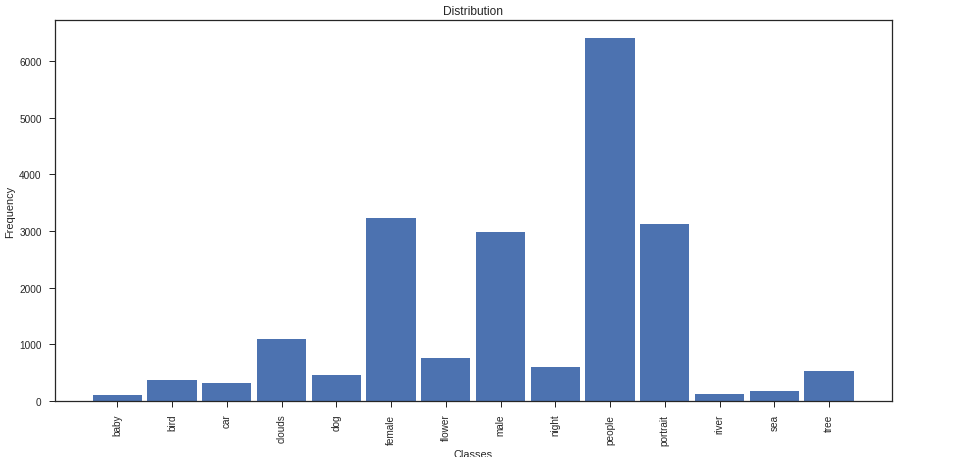
\includegraphics[width=0.6\linewidth]{images/distribution}
		\caption{Distribution of the classes}
		\label{fig:distribution-classes}
	\end{center}
\end{figure}

The main consequence of this problem is that the network could have difficulties to predict correctly the classes with few examples in the training set. Our \textbf{solution} was to find a good threshold for the predictions. Each model that we tried has as final output a fully connected layer with 14 neurons (because we have 14 different classes). The activation function used in this layer is the sigmoid. So, finding the right threshold helps the model out to make good predictions. The idea was to request a minor activation for neurons that represent classes with few examples. Vice versa for the classes with many examples. \\
We started considering as a good threshold the proportion of the data in the training set. For example, if the class 'bird' is the label of the 30\% of the dataset the started threshold for that class is 0.3 (so to predict 1 for this class the output of the neuron should be higher respect to this value). Notice that we have adjusted a bit this threshold in order to have better accuracy than recall. Our idea was to make the predictions when there is an high activation of the corresponding neuron.

\subsection{Batching and scaling}

The chosen batch size is 64 samples. Since we trained on the 90\% of the dataset (180000 images), 64 samples seem reasonable because it allows both to have some updates and good training speed for all the models. Since we are using the \textbf{Adam optimizer} a good learning rate is always found. So, the model requires less optimization step. \\
To improve the results we applied some transformations to the images (i.e. RandomHorizontalFlip and RandomRotation).